\documentclass{beamer}
  \usepackage[english]{babel}
  \usepackage[utf8]{inputenc}
  \usepackage{times}
  \usepackage{amsmath,amsthm, amssymb}
  \boldmath
  
  \usetheme{I6pd}
  %\usetheme{Dreuw}
  \usepackage[orientation=portrait,size=a0,scale=1.4]{beamerposter}


%%% footnote bug https://tex.stackexchange.com/questions/191614/adding-a-frame-footnote-in-beamerposter-creates-blank-page-at-beginning %%%

%%% macro %%%

\usepackage{amsfonts,amssymb}
\usepackage{graphicx}
\usepackage{epic}
\usepackage{qcircuit}
\usepackage{physics}
\usepackage[normalem]{ulem}

%%%%%%%%%%%%%%%%%%%%%%%%%%%%%%%%%%%%%%%%%%%%%%%%%%%%%%%%%%%%%%%%%%%%%%%%%%%%%%%
% Definitions

\newcommand{\<}{\langle}
\renewcommand{\>}{\rangle}

\newcommand{\be}{\begin{equation}}
\newcommand{\ee}{\end{equation}}
\newcommand{\bea}{\begin{eqnarray}}
\newcommand{\eea}{\end{eqnarray}}

%%%%%%%%%%%%%%%%%%%%%%%%%%%%%%%%%%%%%%%%%%%%%%%%%%%%%%%%%%%%%%%%%%%%%%%%%%%%%%%

%%% Info %%%

\title{\Large Quantum Computing, an Introduction with Grover's Search}
\author[Yan-Tong Lin]{Yan-Tong Lin {\small Advisor: Ming-Hsuan Kang}}
\institute[National Chiao Tung University]{{Department of Computer Science}, {National Chiao Tung University}, {Taiwan}}
\date{Individual Study I, December 30, 2020}

%%%%%%%%%%
\begin{document}
\begin{frame}
\vfill
    \begin{block}{Introduction}
        Quantum computation differs from its classical counterpart in a fundamental way. With proper algorithm design, it is known that exponential speedups can be acquired in certain problems. With the advance of quantum hardware technology, the need for efficient quantum algorithms is rising.
        \newline\newline
        In this poster, we aim to introduce some fundamental concepts in quantum computing with the quantum circuit model and some examples. We start by walking through circuit model for classical computation. Then the mathematical formulation of quantum mechanics related to quantum computing is explained, which is used to present the quantum circuit model. Followed by an example showing the power of quantum parallelism --- Deutsch-Jozsa Algorithm. Finally, Grover's search algorithm is introduced to show a quadratic speedup on unstructured search problems. 
    \end{block}
\vfill
    %%%%% No Clolumn %%%%%%%%%
    \begin{columns}[t]
    \begin{column}{.48\linewidth}
        \begin{block}{Classical Circuit Model}

            \begin{itemize}
                \item Bits are used to store information
                    \begin{itemize}
                        \item e.g. $0001$ as $1$, $0101$ as $5$
                    \end{itemize}
                \item Gates are used to manipulate them
                    \begin{itemize}
                        \item e.g. $NAND$ gate
                        \item one can show that $NAND$ can achieve universal computation
                    \end{itemize}
                \item We model physical phenomenon to do these
            \end{itemize}
            
            \begin{figure}
                \centering
                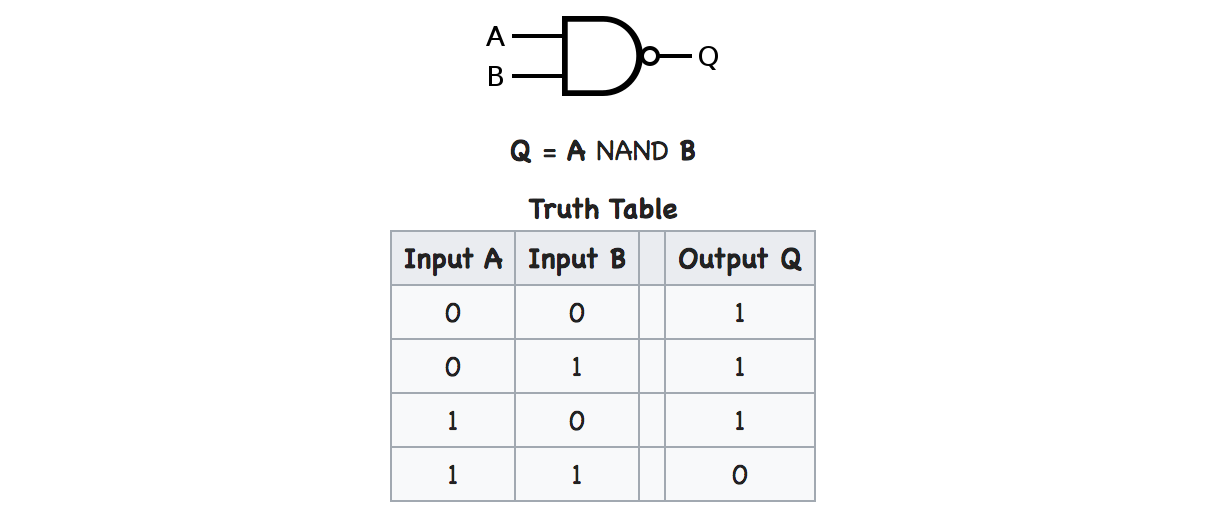
\includegraphics[width=0.5\textwidth]{nand.png}
                \caption{NAND gate and its truth table}
                \label{fig:nand}
            \end{figure}
        
        \end{block}
        

        \begin{block}{Postulates of Quantum Mechanics}
        In the past decades, physicists discover that Nature is "quantum".
                \begin{itemize}
                    \item States of Systems are Unit Vectors in Hilbert Spaces
                    \item Evolutions are linear transforms on the Hilbert space which map states to states.
                    \item Measurements are Collections of Operators
                    \item States of a Compositional System are Tensor Products of States of Component Systems
                \end{itemize}
        \end{block}
        
        \begin{block}{Qubit}

            \begin{itemize}
                \item States of Systems are Unit Vectors in Hilbert Spaces
                \item qubit: $|0\>, |1\>$ 
                \item superpostion: $\alpha|0\>+\beta|1\>, |\alpha|^2+|\beta|^2=1$
            \end{itemize}
            
            \begin{figure}
                \centering
                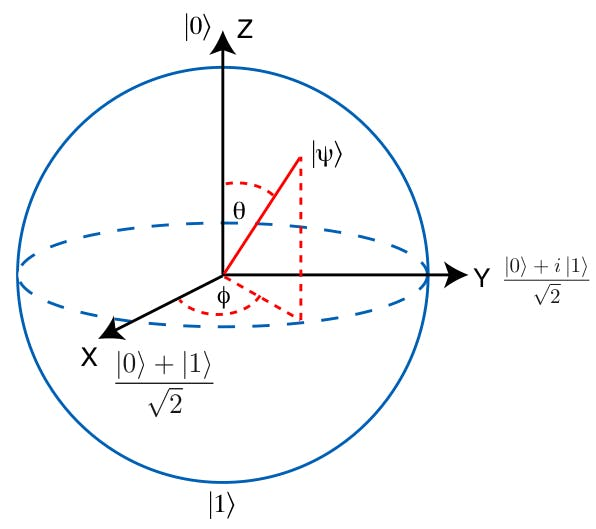
\includegraphics[width=0.4\columnwidth]{bloch.jpg}
                \caption{Bloch Sphere: $|\psi\> = e^{i\delta}(\cos\frac\theta2|0\>+e^{i\phi}\sin\frac\theta2|1\>)$}
                \label{fig:bloch}
            \end{figure}
        
        \end{block}
    
    \begin{block}{Quantum Gates}
    \begin{itemize}
        \item Evolutions are linear transforms on the Hilbert space which map states to states.
        \item Norm-Preserving + Linear $\implies$ Unitary 
        \item Functions on one qubit: Members of $SU(2) \cong SO(3)$
        \item Like in classical computation, it can be shown that there exists finite universal gate sets.
    \end{itemize}

\end{block}
    
    \end{column}
    %%%%%% SEP: COLUMN %%%%%%%%%%%
    %%%%%% SEP: COLUMN %%%%%%%%%%%
    %%%%%% SEP: COLUMN %%%%%%%%%%%
    \begin{column}{.48\linewidth}
\begin{block}{Deutsch-Jozsa Algorithm}

\footnotesize

$f:\{0,1\}^n \to \{0,1\}$ is either balanced or constant.
Given $O_f(|x, y\>) = |x, y\oplus f(x)\>$ as black boxes, judge if $f$ is constant.

\begin{itemize}
\item It requires $O(2^n)$ queries of $f$ for a classical circuit to judge
\item quantum: $O(1)$ query of $O_f$
\end{itemize}

\begin{align*}
 \Qcircuit @C=1em @R=.7em {
  \lstick{\ket{0}} & /^n \qw & \gate{H^{\otimes n}} & \multigate{1}{O_f} & \gate{H^{\otimes n}}	& \meter & \cw \\
  \lstick{\ket{1}} & \qw     & \gate{H}             & \ghost{U_f}        & \qw
 }
\end{align*}


$$\vert \psi_0 \rangle = \vert0\rangle^{\otimes n} \vert 1\rangle$$
$$\vert \psi_1 \rangle = \frac{1}{\sqrt{2^{n+1}}}\sum_{x=0}^{2^n-1} \vert x\rangle \left(|0\rangle - |1 \rangle \right)$$
$$
    \begin{aligned}
    \lvert \psi_2 \rangle  
        & = \frac{1}{\sqrt{2^{n+1}}}\sum_{x=0}^{2^n-1} \vert x\rangle (\vert f(x)\rangle - \vert 1 \oplus f(x)\rangle) \\  
        & = \frac{1}{\sqrt{2^{n+1}}}\sum_{x=0}^{2^n-1}(-1)^{f(x)}|x\rangle ( |0\rangle - |1\rangle ) 
    \end{aligned}
$$
$$
\begin{aligned}
    \lvert \psi_3 \rangle 
        & = \frac{1}{2^n}\sum_{x=0}^{2^n-1}(-1)^{f(x)}
            \left[ \sum_{y=0}^{2^n-1}(-1)^{x \cdot y} 
            \vert y \rangle \right] \\
        & = \frac{1}{2^n}\sum_{y=0}^{2^n-1}
            \left[ \sum_{x=0}^{2^n-1}(-1)^{f(x)}(-1)^{x \cdot y} \right]
            \vert y \rangle
\end{aligned}
$$

Now consider $|y\>=|0\>$
$$
\frac{1}{2^n}\sum_{x=0}^{2^n-1}(-1)^{f(x)}(-1)^{x \cdot 0}
            \vert 0 \rangle
$$
We get the first register measures $|0\>^{\otimes n} \iff f $ is constant

\end{block}

%%%%


\begin{block}{Grover's Search}

\footnotesize

Given a set $X$ of $N$ items and a function $f : X \to \{0,1\}$, \newline
suppose there are $M=\epsilon N$ out of $N$ items satisfy $f(x)=1$. \newline
Find an instance $x \in S$ such that $f(x)=1$.
\begin{itemize}
    \item For classical algorithms, $O(N)$-time is required to get an instance with high probability.

    \item For quantum algorithms, assume an oracle $U_\omega$ is given such that 
$$
U_\omega|x\rangle = (-1)^{f(x)}|x\rangle .
$$
    With Grover's Search, $O(\sqrt{N})$-time is suffice.
\end{itemize}

Represent uniform state vector by l.c. of uniform "good" and uniform "bad" vectors. \newline
$|s\rangle = \sqrt{\frac{1}{N}}\sum_{x} |x\rangle$ \newline
$|\omega\rangle = \sqrt{\frac{M}{N}}\sum_{x \in f^{-1}(1)} |x\rangle$ \newline
$|s^{'}\rangle = \sqrt{\frac{N-M}{N}}\sum_{x \not \in f^{-1}(1)} |x\rangle$ \newline
then $|s\rangle = \sin\frac\theta2|\omega\rangle + \cos\frac\theta2|s^{'}\rangle$ where $\sin\frac\theta2 = \sqrt{\frac{M}{N}}$


$$U_\omega = I - 2|\omega\rangle\langle \omega|$$
$$U_s = 2 \left|s\right\rangle \left\langle s\right| - I$$

\begin{align*}
 \Qcircuit @C=1em @R=.7em {
                   &         &                      &                         &                      & \ustick{\text{Grover diffusion operator $U_s$}} \\
  \lstick{\ket{0}} & /^n \qw & \gate{H^{\otimes n}} & \multigate{1}{U_\omega} & \gate{H^{\otimes n}} & \gate{2 \ket{0^n}\bra{0^n} - I_n}         & \gate{H^{\otimes n}} & \qw & \cdots & & \meter & \cw \\
  \lstick{\ket{1}} & \qw     & \gate{H}             & \ghost{U_\omega}        & \qw                  & \qw                                       & \qw                  & \qw & \cdots & \\
                   &         &                      &                         &                      & \dstick{\text{Repeat $O(\sqrt{N})$ times}}
  \gategroup{2}{5}{2}{7}{.7em}{^\}}
  \gategroup{2}{4}{3}{10}{.7em}{_\}}
 }
\end{align*}

\begin{figure}
    \centering
    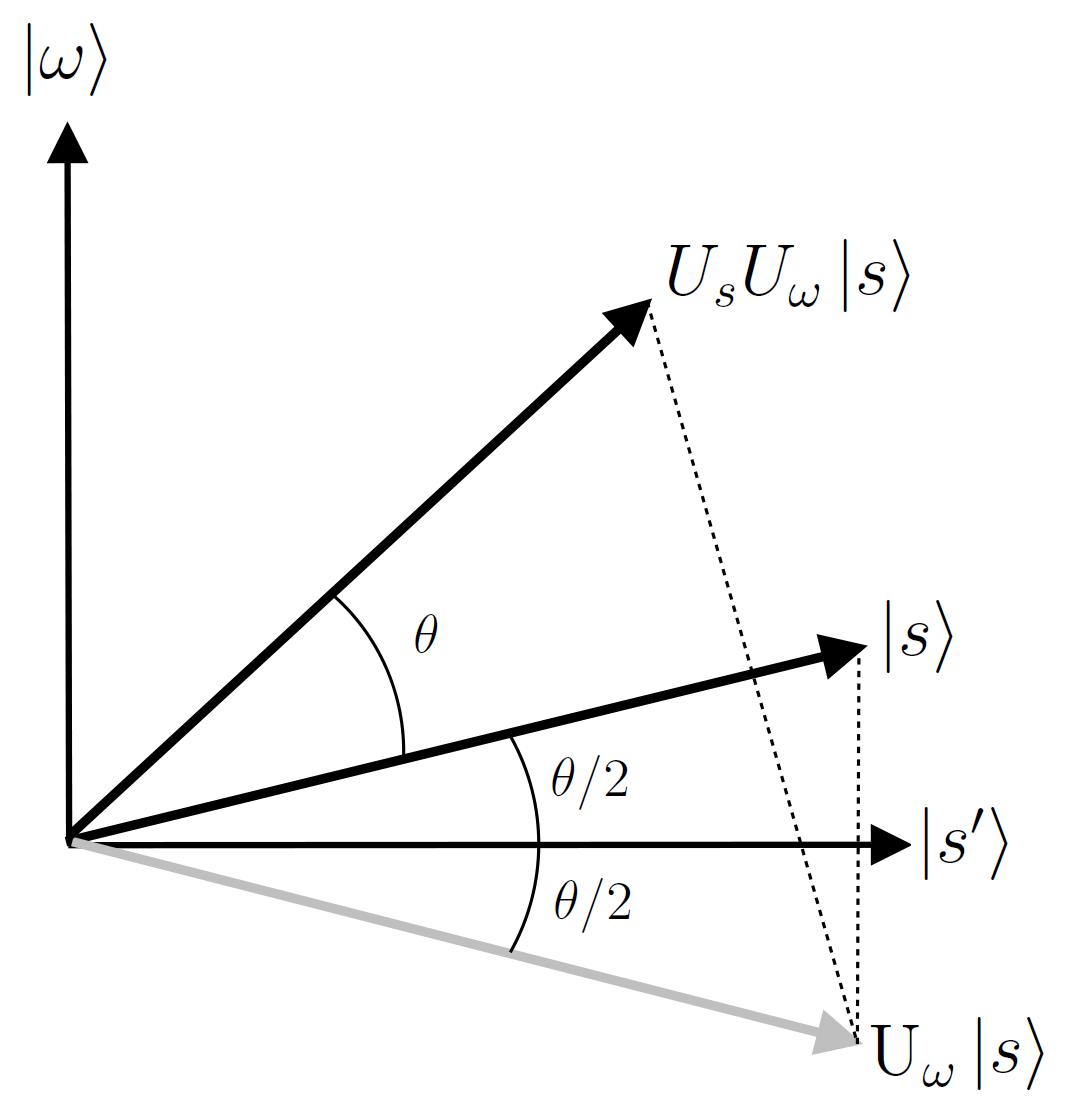
\includegraphics[width=0.3\columnwidth]{grover_geo.png}
    \label{fig:grover_geo}
\end{figure}

We want to stop when the state vector passes close to $|\omega \rangle$. 
$r = \#\text{round} \approx \pi \sqrt {N}/4$ is the first $r$ we can get a high probability.

\end{block}


        \end{column}
    \end{columns}

\end{frame}
\end{document}


%%%%%%%%%%%%%%%%%%%%%%%%%%%%%%%%%%%%%%%%%%%%%%%%%%%%%%%%%%%%%%%%%%%%%%%%%%%%%%%%%%%%%%%%%%%%%%%%%%%%